%%%%%%%%%%%%%%%%%%%%%%%%%%%%%%%%%%%%%%%%%%%%%%%%%%%%%%%%%%%%%%%%%%%%%%%%%
% ARTICLE ABOUT FATE OF SYNONYMOUS MUTATIONS IN HIV
%%%%%%%%%%%%%%%%%%%%%%%%%%%%%%%%%%%%%%%%%%%%%%%%%%%%%%%%%%%%%%%%%%%%%%%%%
\documentclass[rmp, twocolumn]{revtex4}
%%%%%%%%%%%%%%%%%%%%%%%%%%%%%%%%%%%%%%%%%%%%%%%%%%%%%%%%%%%%%%%%%%%%%%%%%
%%%%%%%%%%%%%%%%%%%%%%%%%%%%%%%%%%%%%%%%%%%%%%%%%%%%%%%%%%%%%%%%%%%%%%%%%
\newcommand{\Author}{Fabio~Zanini and Richard~A.~Neher}
\newcommand{\env}{\textit{env}}

\newcommand{\Title}{Deleterious synonymous mutations hitchhike to high frequency in HIV \env~evolution}
\newcommand{\Keywords}{{HIV}, {synonymous}, {population genetics}}
\usepackage[english]{babel}
\usepackage[utf8x]{inputenc}
\usepackage{amsmath,amsfonts,amssymb,eucal,eurosym,textcomp}
\usepackage{color}
\usepackage{graphicx}
\usepackage[caption=false]{subfig}
\usepackage{natbib}
\usepackage{pslatex}
\usepackage[colorlinks,linkcolor=red,citecolor=red]{hyperref}
\hypersetup{pdfauthor={\Author}, pdftitle={\Title}, pdfkeywords={\Keywords}}
%%%%%%%%%%%%%%%%%%%%%%%%%%%%%%%%%%%%%%%%%%%%%%%%%%%%%%%%%%%%%%%%%%%%%%%%%
\graphicspath{{./figures/}}
%%%%%%%%%%%%%%%%%%%%%%%%%%%%%%%%%%%%%%%%%%%%%%%%%%%%%%%%%%%%%%%%%%%%%%%%%
%\DeclareMathOperator\de{d\!}
\newcommand{\comment}[1]{\textit{\textcolor{red}{#1}}}
\newcommand{\mut}{\mu}
\newcommand{\mfit}{\langle F\rangle}
\newcommand{\mexpfit}{\langle e^{F}\rangle}
\newcommand{\ox}{r}
\newcommand{\co}{\rho}
\newcommand{\gt}{g}
\newcommand{\locus}{s}
\newcommand{\locuspm}{t}
\newcommand{\OO}{\mathcal{O}}
\newcommand{\rev}{\textit{rev}}
\newcommand{\FIG}[1]{Fig.~\ref{fig:#1}}
\newcommand{\FIGS}[2]{Figs.~\ref{fig:#1} and~\ref{fig:#2}}
\newcommand{\shankaregion{C2-C5}

%%%%%%%%%%%%%%%%%%%%%%%%%%%%%%%%%%%%%%%%%%%%%%%%%%%%%%%%%%%%%%%%%%%%%%%%%
%%%%%%%%%%%%%%%%%%%%%%%%%%%%%%%%%%%%%%%%%%%%%%%%%%%%%%%%%%%%%%%%%%%%%%%%%
\begin{document}
\title{\Title}
\author{\Author}
\date{\today}
%%%%%%%%%%%%%%%%%%%%%%%%%%%%%%%%%%%%%%%%%%%%%%%%%%%%%%%%%%%%%%%%%%%%%%%%%

\begin{abstract}
\noindent
Intrapatient HIV evolution is governed by selection on the protein level in the
arms race with the immune system (killer T-cells and antibodies). Synonymous
mutations do not have an immunity-related phenotype and are often assumed to be
neutral. In this paper, we show that synonymous changes in epitope-rich regions
are often deleterious but still reach high frequencies.  We analyze time
series of viral sequences from the \shankaregion~part of {\it env} within individual
hosts and observe that synonymous derived alleles rarely fix in the
viral population. Simulations suggest that such synonymous mutations
have a (Malthusian) selection coefficient of the order of $-0.001$, and that
they are brought up to high frequency by hitchhiking with neighboring beneficial
nonsynonymous alleles. We detect a negative correlation between fixation of an allele and
its involvement in RNA stem-loop structures.
Deleterious synonymous mutations are observed in other parts of the HIV genome, in which
selective sweeps are less dense and hitch-hiking not as strong.
\end{abstract}

\end{abstract}
\maketitle

\section{Introduction}

HIV evolves rapidly within a single host during the course of the infection.
This evolution is driven by strong selection imposed by the host immune system
via killer T cells (CTLs) and neutralizing antibodies
(ABs)~\citep{pantaleo_immunopathogenesis_1996} and facilitated by the high
mutation rate of HIV~\citep{mansky_lower_1995}. When the host develops a CTL or
AB response against a particular HIV epitope, mutations in the viral genome that
reduce or prevent recognition of the epitope frequently emerge. Escape mutations
in epitopes targeted by CTLs typically evolve during early infection and spread
rapidly through the population~\citep{mcmichael_immune_2009}. During chronic
infection, the most rapidly evolving part of the HIV genome are the so called
variable loops of the envelope protein gp120, which need to avoid recognition by
neutralizing ABs.  Mutations in \env~, the gene encoding for gp120, spread
through the population within a few months (see \figurename~\ref{fig:aft}, solid
lines).  The (Malthusian) effect size of these beneficial mutations is of the
order of $s_a \sim 0.01$~\citep{neher_recombination_2010}.

These escape mutations are strongly selected for their effect on the amino acid
sequence of the viral proteins. Conversely, synonymous mutations are commonly
used as approximate neutral markers in studies of viral evolution. Neutral
markers are very useful in practice, because they can be used to make inferences
about the stochastic forces driving evolution~\citep{yang_statistical_2000}.
The viral genome, however, needs to satisfy further constraints in addition to
immune escape, such as efficient processing and translation, nuclear export, and
packaging into the viral capsid: all these processes operate at the RNA level
and are sensitive to synonymous changes. A few functionally important RNA
elements are well characterized. For example, a certain RNA sequence in the HIV
genome, called \rev{} response element (RRE), enhances nuclear export of viral
transcripts~\citep{fernandes_hiv-1_2012}. Another well studied case is the
interaction between viral reverse transcriptase, viral ssRNA, and the host
tRNA$^\text{Lys3}$: the latter is required for priming reverse transcription
(RT) and bound by a specifical pseudoknotted RNA structure in the viral 5'
untranslated region~\citep{barat_interaction_1991, paillart_vitro_2002}.
Nucleotide-level fitness effects have been observed beyond RNA structure as
well. Recent studies have shown that genetically engineered HIV strains with
skewed codon usage bias (CUB) patterns towards more or less abundant tRNAs
replicate better or worse, respectively~\citep{ngumbela_quantitative_2008,
li_codon-usage-based_2012}. A similar conclusion has been reached about
influenza, and codon-pessimized influenza strains have been shown to be good
live attenuated vaccines in mice~\citep{mueller_live_2010}. Purifying selection
beyond the protein sequence is therefore expected, while it seems reasonable
that the bulk of positive selection through the immune system be restricted to
amino acid sequences.

%SYNONYMOUS CONSERVATION. DO WE HAVE A PLOT OF GENOME WIDE CONSERVATION, MAYBE
%FOR SUPPLEMENT? YES

In this paper, we characterize the dynamics of synonymous mutations in \env{}
and show that a substantial fraction of these mutations is deleterious. We
further show that, although such synonymous mutations cannot be used as neutral
markers, the degree to which they hitchhike with nearby nonsynonymous mutations
is very informative. Their ability to hitchhike for extended times, which is a
core requirement for our analysis, is rooted in the small recombination rate of
HIV~\citep{neher_recombination_2010, batorsky_estimate_2011}. Extending the
analysis of fixation probabilities to the nonsynonymous mutations, we show that
time dependent selection or strong competition of escape mutations inside the
same epitope are necessary to explain the observed patterns of fixation and
loss.

\section{Results}

The central quantity we investigate is the probability of fixation of a
mutation, conditional on its population frequency.  A neutral mutation
segregating at frequency $\nu$ has a probability $P_\text{fix}(\nu) = \nu$ to
spread through the population and fix; in the rest of the cases, i.e. with
probability $1-\nu$, it goes extinct. This is a simple consequence of the fact
that (a) exactly one of the $N$ individuals in the current population will be
the common ancestor of the entire future population at a particular locus and
(b) this ancestor has a probability $\nu$ of carrying the mutation, see
illustration in \FIG{fixp}.  Deleterious or beneficial mutations fix less or
more often than neutral ones, respectively. Time series sequence data enable a
direct observation of both the current frequency $\nu$ of any particular
mutation and its future fate (fixation or extinction). They therefore represent
a simple way to investigate average properties of different classes of
mutations. 

\subsection{Synonymous polymorphisms in \env, C2-V5 are mostly deleterious}

\FIG{aft} shows time series data of the frequencies of all mutations observed
\env~, C2-V5, in patient p8~\citep{shankarappa_consistent_1999}. Despite many
synonymous mutations reaching high frequency (dashed lines), very few fix. This
observation is quantified in panels \FIG{fixp1} and \ref{fig:fixp2}, which
stratify the data of 7 (resp. 10) patients according to the frequency at which
different mutations are observed (see methods). Considering all mutations in a
frequency interval around $\nu_0$ at some time $t_i$, we calculate the fraction
that is found at frequency 1, at frequency 0, or at intermediate frequency at
later times $t_f$. Plotting these fixed, lost, and polymorphic fraction against
the time interval $t_f-t_i$, we see that most synonymous mutations segregate for
roughly two years and are lost much more frequently than expected. The long-time
probability of fixation versus extinction is shown as a function of the initial
frequency $\nu_0$ in panel~\ref{fig:fixp2} (red line). In contrast to synonymous
mutations, the nonsynonymous seem to follow more a less the neutral expectation
(blue line) -- a point to which we will come back below. 

\begin{figure}
\begin{center}
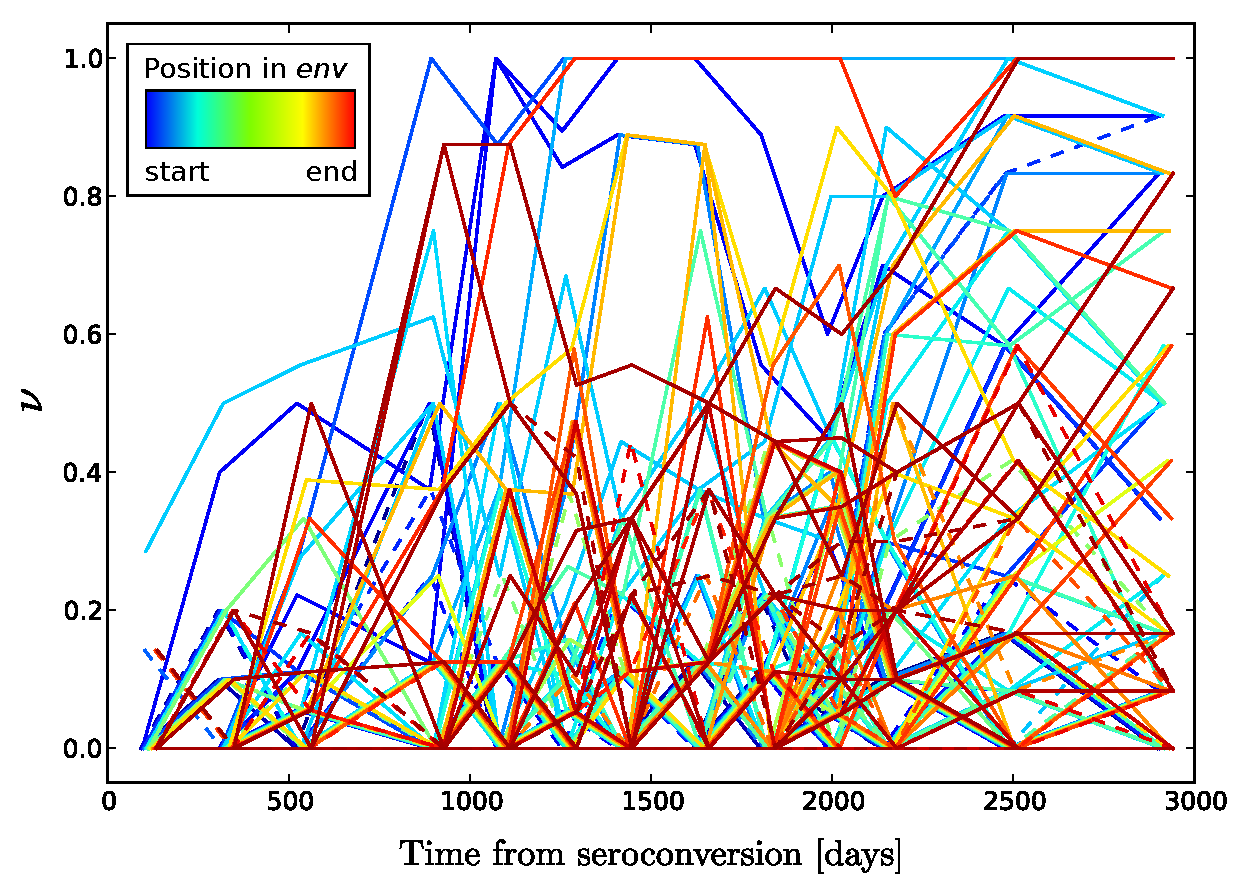
\includegraphics[width=\linewidth]{Shankarappa_allele_freqs_trajectories_syn_nonsynp8}
\caption{Synonymous mutations rarely fix in \env, C2-V5: mutation frequency
 trajectories observed in patient 8~\cite{shankarappa_consistent_1999};
 Nonsynonymous and synonymous mutations are shown as solid and dashed lines,
 respectively. Colors indicate the position of the site along the C2-V5 region
 (red to blue) MAYBE MAKE FIGURE WITH SYNONYMOUS AND NONSYN
 SEPARATELY. While nonsynonymous mutations frequently fix, very few synonymous
mutations do even though they are frequently observed at intermediate
frequencies.}
\label{fig:aft}
\end{center}
\end{figure}

\citet{bunnik_autologous_2008} present a longitudinal dataset on the entire
\env~gene of 3 patients at $\sim 5$ time points with approximately 5-20
sequences each (see methods). Repeating the above analysis separately on the
C2-V5 region studied above and the remainder of \env~ reveal striking
differences (see \FIG{fixp}). Within C2-V5, this data fully confirms the
observations made in the data set by \citet{shankarappa_consistent_1999} (red
line). In the remainder of \env, however, observed synonymous mutations behave
as if they were neutral (orange line). 

%ARE OBSERVED SYNONYMOUS MUTATIONS OUTSIDE C2-V5 NEUTRAL? (?? SOME!)
%DOES LOSS/FIX CORRELATE WITH CONSERVATION? YES.
%MAYBE WE COULD HAVE ONE -- COMPLETELY CIRCULAR -- FIGURE SHOWING LOSS/FIX VS CONSERVATION: SUPPLEMENTARY?
%CAN WE LOOK AT THE AVERAGE LEVEL OF CONSERVATION STRATIFIED BY MAX FREQ? TRICKY: the maximal freq is achieved by hitchhiking...

These observations suggest that many of the synonymous polymorphisms in the part
of \env~that includes the hypervariable regions are deleterious, while outside
this regions polymorphisms are mostly roughly neutral. Note that this does not imply that all 
synonymous mutations are neutral -- only those mutations observed at high frequencies tend 
to be neutral.

\begin{figure}
\begin{center}
\subfloat{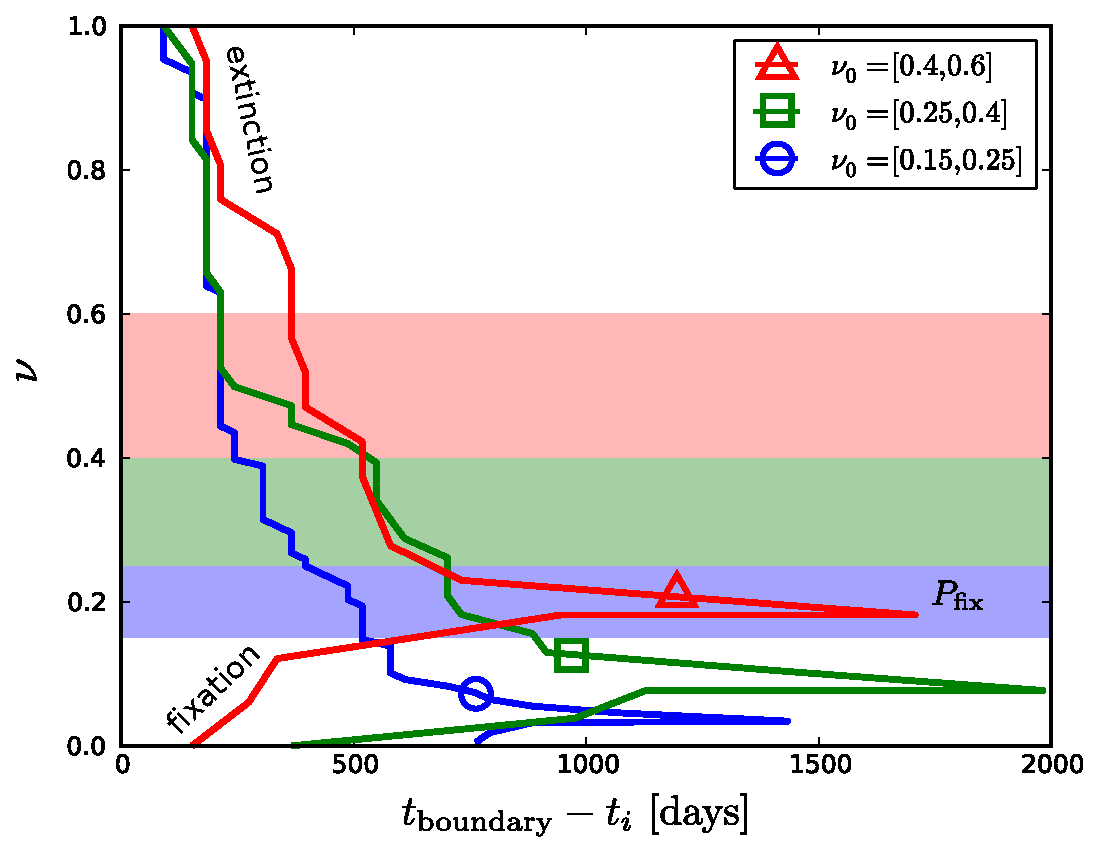
\includegraphics[width=0.9\linewidth]{Shankarappa_fix_loss_dt_times}
\label{fig:fixp1}}\\
\subfloat{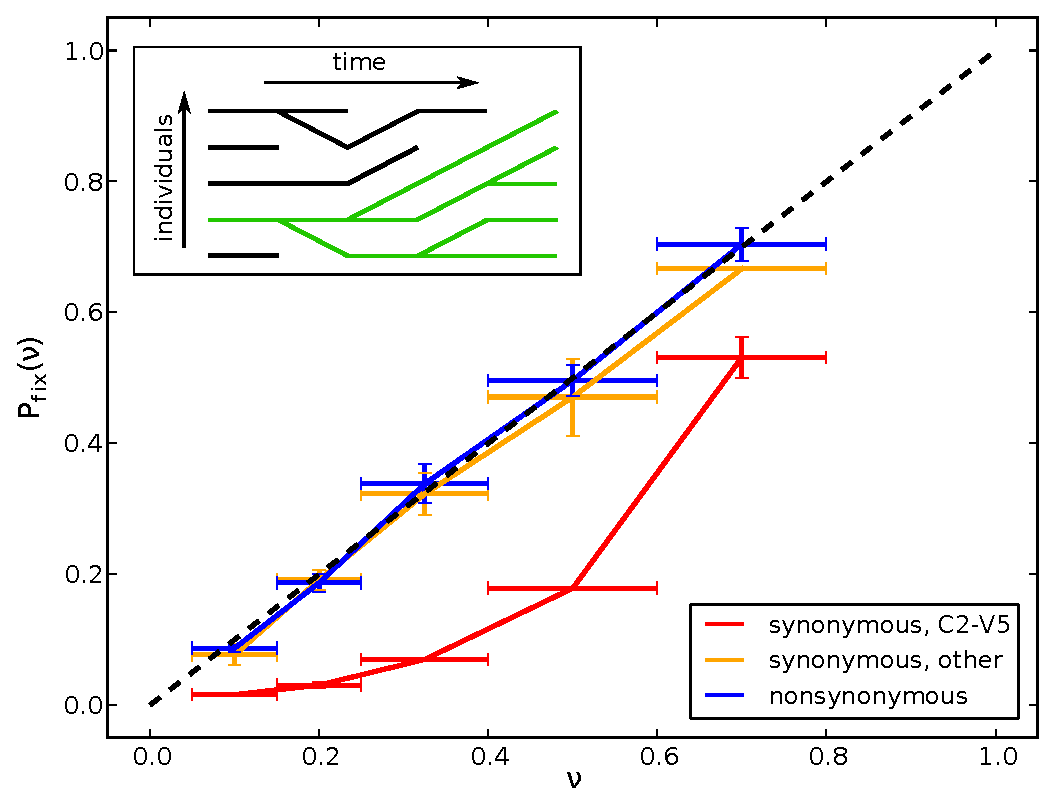
\includegraphics[width=0.9\linewidth]{Bunnik2008_fixmid_syn_ShankanonShanka}
\label{fig:fixp2}}
\caption{Left panel: time course of loss and fixation of synonymous mutations
 observed in a frequency interval $\nu_0$. The ultimate fraction of synonymous
 mutations that fix as a function of intermediate frequency $\nu_0$ is the
 fixation probability.  Right panel: fixation probability of derived synonymous
alleles is strongly suppressed in C2-V5 versus other parts of the {\it env}
gene, and of nonsynonymous ones. Data from
Refs.~\cite{shankarappa_consistent_1999, bunnik_autologous_2008}.}
\label{fig:fixp}
\end{center}
\end{figure}

\subsection{Synonymous mutations in C2-V5 tend to disrupt conserved RNA stems}

One possible {\it a priori} explanation for lack of fixation of synonymous
mutations in C2-V5 are  secondary structures in the viral RNA. If any RNA
secondary structures are relevant for HIV replication, mutations in nucleotides
involved in those base pairs are expected to be deleterious and to revert
preferentially. Many functionally important secondary structure elements have
been characterized, including  the RRE~\citep{fernandes_hiv-1_2012} and the 5'
UTR pseudoknot interacting with the host
tRNA$^\text{Lys3}$~\citep{barat_interaction_1991, paillart_vitro_2002}. It has
been suggested early on that parts of the viral genome that has the potential to
form stems is better conserved than the
remainder~\citep{forsdyke_reciprocal_1995}.

Recently, the propensity of nucleotides of the HIV genome to form base pairs has
been measured using the SHAPE assay (a biochemical reaction preferentially
altering unpaired bases)~\citep{watts_architecture_2009}. The SHAPE assay has
shown that the variable regions V1 to V5 tend to be unpaired, while the
conserved regions between those variable regions form stems. We partition all
synonymous alleles observed at intermediate frequencies above 10-15\% depending
on their final destiny (fixation or extinction). Subsequently, we align our
sequences to the reference NL4-3 strain used in
ref.~\citep{watts_architecture_2009} and assign them SHAPE reactivities. As
shown in \FIG{SHAPEA} in a cumulative histogram, the reactivities of fixed
alleles (red line) are systematically larger than of alleles that are doomed to
extinction (blue line) (Kolmogorov-Smirnov test, $P\approx
2~\text{\textperthousand}$). In other words, alleles that are likely to be
breaking RNA helices are also more likely to revert and finally be lost from the
population. As a control, the average over non-observed but potentially
available polymorphisms lies between the two curves (green line), as expected
(because only some of them will be helix breakers). Furthermore, as a
complementary analysis, we split the synonymous mutations in the extended V1-V5
region further into conserved and variable regions and found that the biggest
depression in fixation probability is observed in the conserved stems, while the
variable loops show little deviation from the neutral signature, see
\FIG{SHAPEB}. 

In addition to RNA secondary structure, we have considered other possible
explanations for a fitness effect of synonymous mutations, in particular codon
usage bias (CUB). HIV is known to prefer A-rich codons over highly expressed
human housekeeping genes~\citep{jenkins_extent_2003}. Moreover, codon-optimized
and -pessimized viruses have recently been generated and shown to replicate
better or worse than wild type strains,
respectively~\citep{li_codon-usage-based_2012, ngumbela_quantitative_2008,
coleman_virus_2008}. We do not find, however, evidence for any contribution of
CUB to the ultimate fate of synonymous alleles. Several lines of thought support
this result. First of all, although codon-optimized HIV seems to perform better
{\it in vitro}, the distance in CUB between HIV and human genes is not shrinking
at the macroevolutionary level. Second, within a single patient, we do not
observe any bias towards more human-like CUB in the synonymous mutations that
reach fixation rather than extinction. Third, it is a common phenomenon for
retroviruses to use variously different codons from their hosts, and CUB effects
on fitness are thought to be so small that divergent nucleotide composition has
been suggested as a possible mechanism for viral
speciation~\citep{bronson_nucleotide_1994}. Fourth, CUB in the V1-C5 region is
not very different from other parts of the HIV genome, whereas the reduced
fixation probability is only observed there. In conclusion, although we cannot
exclude an effect of CUB on fitness as a general rule, we expect it to be a
minor effect in our context.
\begin{figure}
\begin{center}
\subfloat{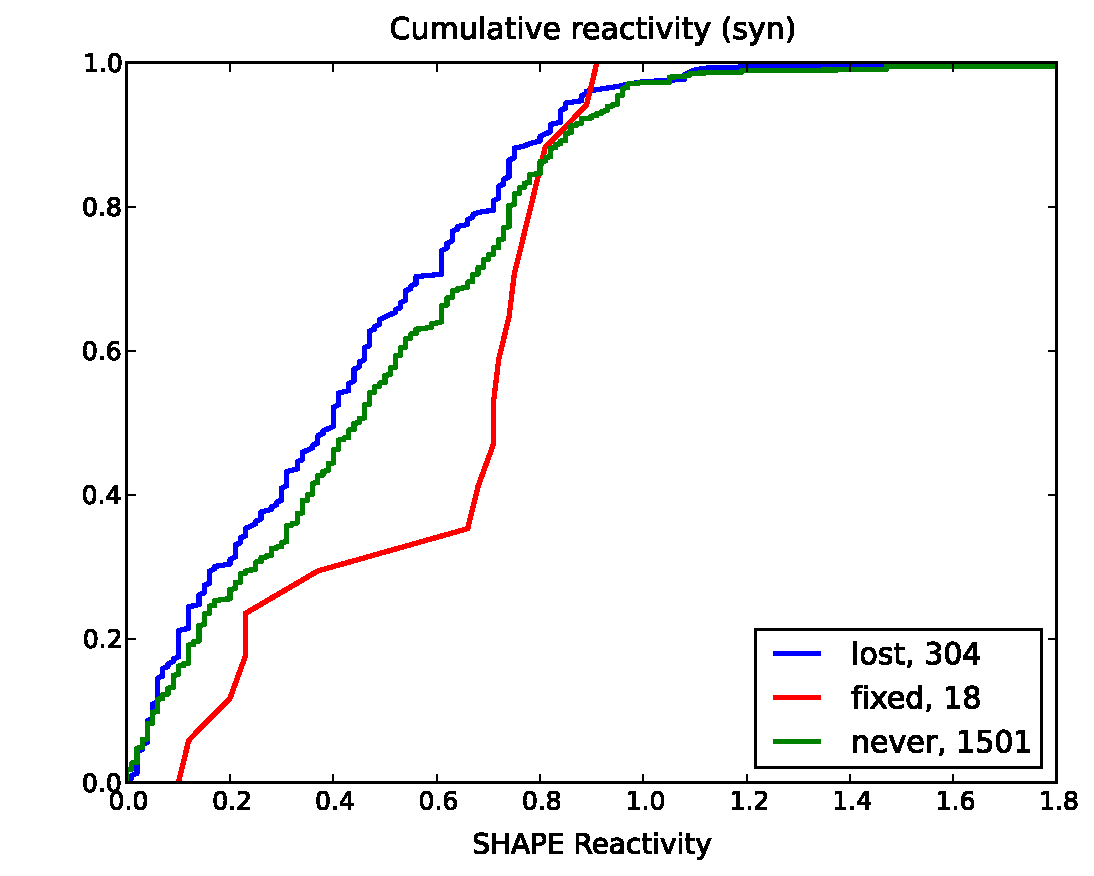
\includegraphics[width=0.9\linewidth]{mixed_Shankarappa_Bunnik2008_Liu_fixation_reactivity_Vandflanking_fromSHAPE}
\label{fig:SHAPEA}}\\
\subfloat{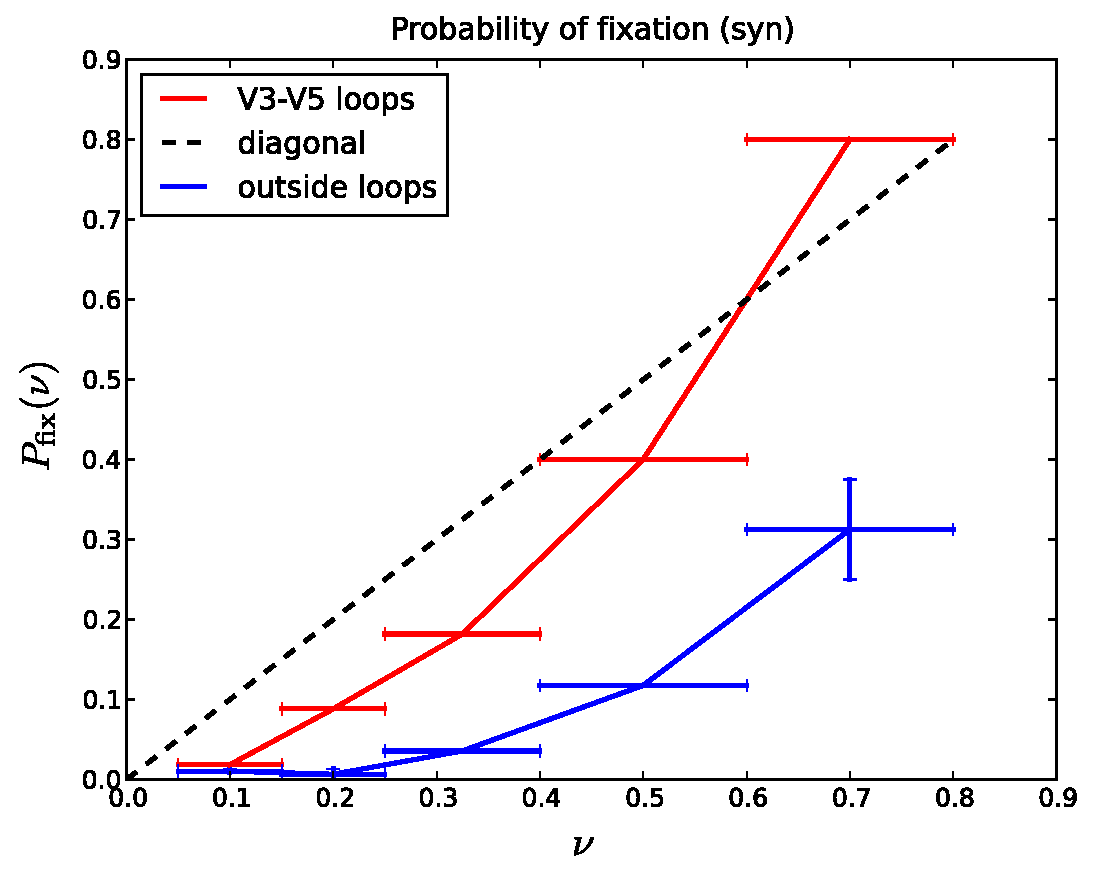
\includegraphics[width=0.9\linewidth]{Shankarappa_fixmid_syn_V_regions.pdf}\label{fig:SHAPEB}}
\caption{Watts et al. have measured the reactivity of HIV nucleotides to {\it
in vitro} chemical attack and shown that some nucleotides are more likely to
be involved in RNA secondary folds. C1-C5 regions, in particular, show
conserved stem-loop structures~\citep{watts_architecture_2009}. We show that
among all derived alleles in those regions reaching frequencies of order one,
there is a negative correlation between fixation and involvement in a base
pairing in a RNA stem (left panel). The rest of the genome does not show any
correlation (right panel). There might be too few silent polymorphisms in the
first place, or the signal might be masked by non-functional RNA
structures. Data from Refs.~\cite{shankarappa_consistent_1999,
bunnik_autologous_2008, liu_selection_2006}.}
\label{fig:SHAPE}
\end{center}
\end{figure}


\subsection{Deleterious mutations are brought to high frequency by hitch-hiking}

While the observation that some fraction of synonymous mutations is deleterious
is not unexpected, it seems odd that we observe them at high population
frequency -- at least in some regions of the genome. The region of \env~ in
which we observe deleterious mutations at high frequency, however, is special in
that it undergoes frequent adaptive changes to evade recognition by neutralizing
antibodies~\cite{williamson_adaptation_2003}. Due to the limited amount of
recombination in HIV~\cite{neher_recombination_2010,batorsky_estimate_2011},
deleterious mutations that are linked to adaptive variants can reach high
frequency~\citep{smith_hitch-hiking_1974}.

The potential for hitchhiking is already apparent from the allele frequency
trajectories in \FIG{aft}, where many mutations appear to change rapidly in
frequency as a flock. Deleterious synonymous mutations can be amplified
exponentially by selection on linked nonsynonymous sites, a process known as
{\it genetic draft}~\citep{gillespie_genetic_2000, neher_genetic_2011}. In order
to be advected to high frequency by a linked adaptive mutation, the deleterious
effect of the mutation has to be substantially smaller than the adaptive effect.
The latter was estimated to be on the order of $s_a = 0.01$ per day~\citep{neher_recombination_2010}.
The approximate magnitude of the deleterious effects can be estimated from
\FIG{fixp1}, that shows the distribution of times for synonymous
alleles to reach the fix or get lost starting from intermediate frequencies. The
typical time to loss is of the order of 500 days. If this loss is driven by the
deleterious effect of the mutation, this corresponds to deleterious effects of
roughly $s_d \sim - 0.002$ per day.

To get a better idea of the range of parameters that are compatible with the
observations and our interpretation, we  perform computer simulations of
evolving viral populations under selection and rare recombination. For this
purpose, we use the recently published package FFPopSim, which includes a module
dedicated to intrapatient HIV evolution~\citep{zanini_ffpopsim:_2012}. We
analyze many combinations of parameters such as population size, recombination
rate, selection coefficient and density of escape mutations, and deleterious effect
of synonymous mutation.

The main result of the simulations is that genetic draft can indeed bring weakly
deleterious mutations to high frequencies and result in a dependence of the
fixation probability on initial frequency that is compatible with observations.
First of all, since neutral mutations are much more likely to rise to high
frequency than deleterious ones, the majority of the synonymous mutations needs
to be slightly deleterious observe a significant reduction of $P_\text{fix}$.
In order to further quantify the reduction in fixation probability, we look at
the difference between the neutral curve ($P_\text{fix}(\nu) = \nu$) and the
measured fixation probability and calculate its area (see inset of
\FIG{simfixpvar}). The minimal and maximal values for this area are zero
(neutral-like curve) and 0.5 (no fixation at all), respectively. The HIV data
correspond to an area under the diagonal of approximately 0.2 for synonymous
changes, and a very small area over the diagonal for nonsynonymous changes.
Various simulation curves are shown in \FIG{simfixpvar}. Then, in
\FIGS{simheat1}{simheat2}, we explore the parameter space: the combinations that
yield areas close to the experimental result are roughly indicated by ellipses.
The two crucial parameters that control the fixation probability are the
following: (a) the deleterious effects of hitchhikers compared to the beneficial
effects of escape mutants, and (b) the density of escape mutations. Intuitively,
a higher density of escape mutations (i.e., epitopes) enables a larger degree of
genetic draft, because escape mutations from different epitopes start to combine
and their effects add up. In \FIG{simheat1}, we show that this is indeed the
case in simulations.

\begin{figure}
\begin{center}
\subfloat{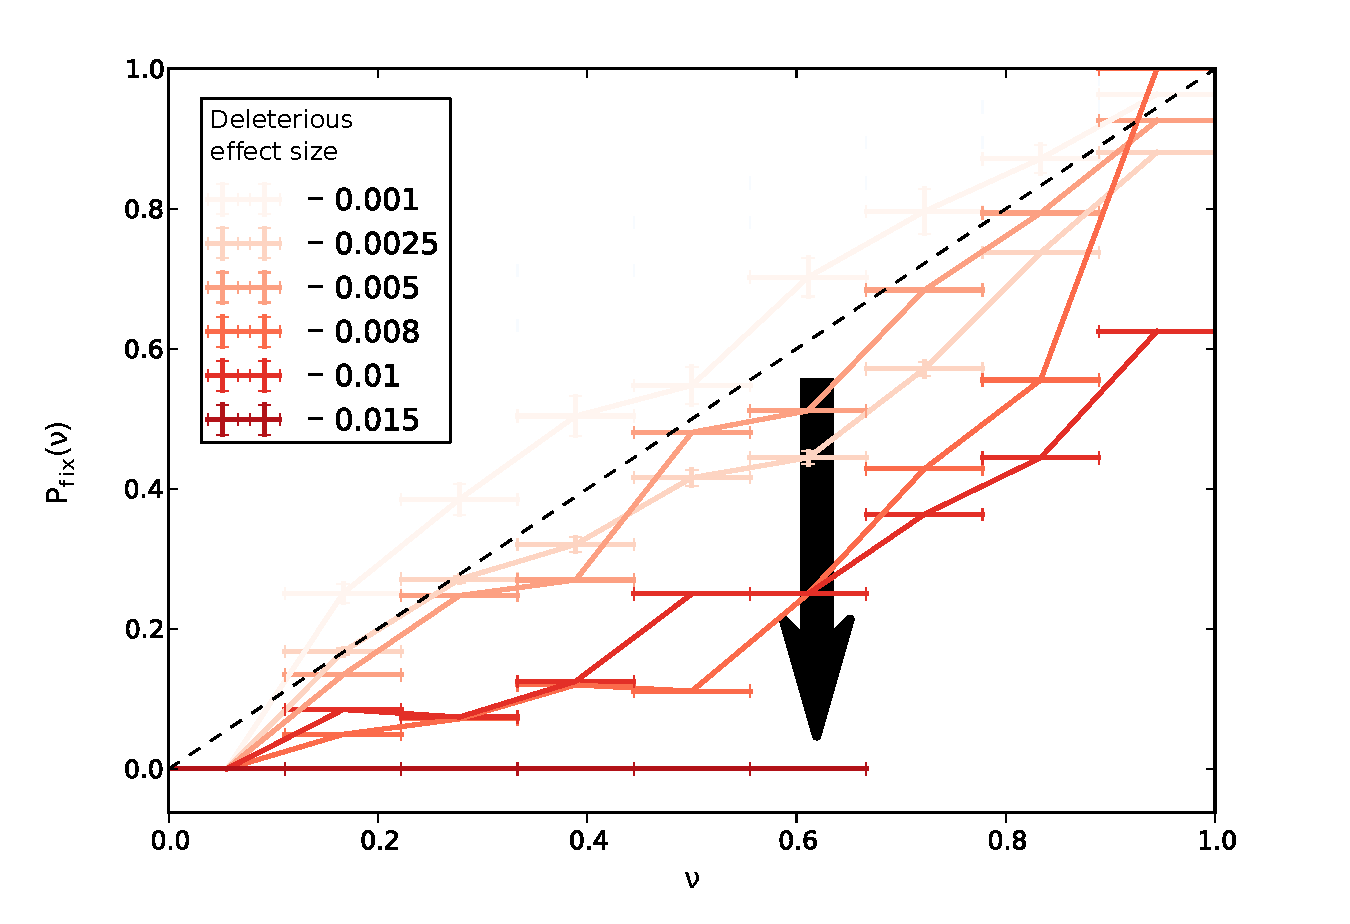
\includegraphics[width=0.9\linewidth]{fixation_loss_shortgenome_distance_ada_frac_del_eff_coi_various.pdf}
\label{fig:simfixpvar}}\\
\subfloat{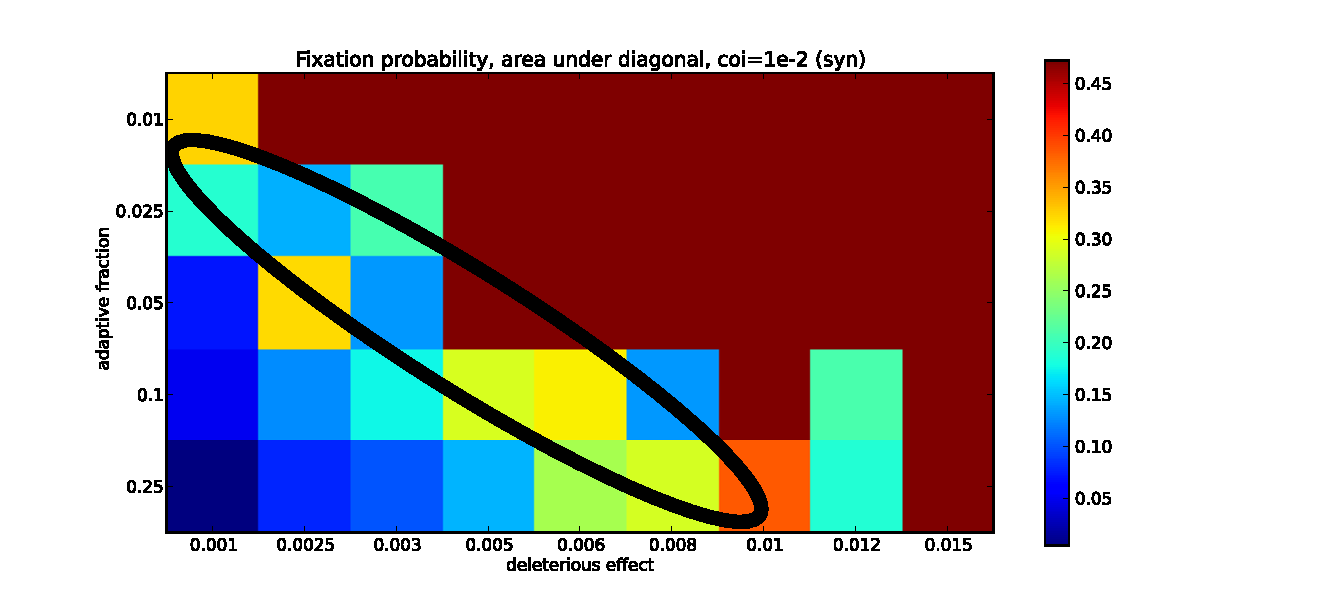
\includegraphics[width=0.9\linewidth]{fixation_loss_shortgenome_area_ada_frac_del_eff_coi_0_01_nescepi_6_heat.pdf}
\label{fig:simheat1}}\\
\subfloat{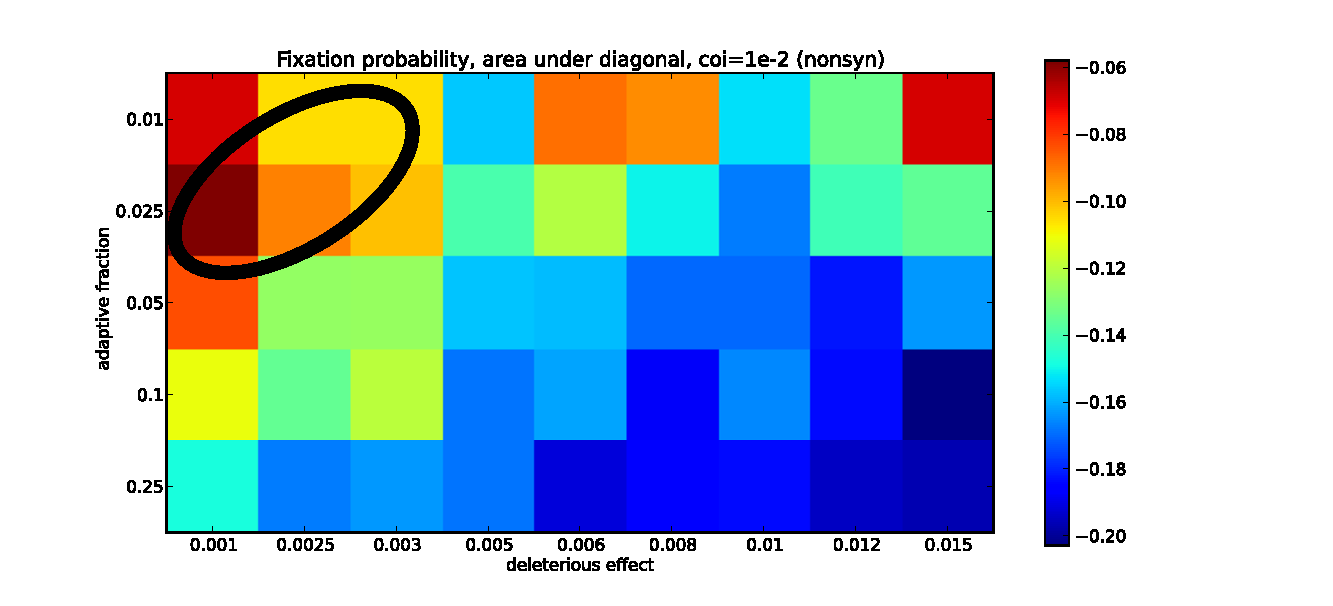
\includegraphics[width=0.9\linewidth]{fixation_loss_shortgenome_area_ada_frac_del_eff_coi_0_01_nescepi_6_nonsyn_heat.pdf}
\label{fig:simheat2}}
\caption{\comment{USE A GOOD FIG WITH THE CORRECT $s_a$!} The depression in $P_\text{fix}$ depends on the deleterious effect size
 of the synonymous alleles (panel A). Simulations on the escape competition
 scenario show that the density of selective sweeps and the size of the
 deleterious effects of synonymous mutations are the main driving forces of the
 phenomenon. A convex fixation probability is recovered, as seen in the data,
 along the diagonal (panel B): more dense sweeps can support more deleterious
 linked mutations. The density of sweeps is limited, however, by the
 nonsynonymous fixation probability, which is quite close to neutrality (panel
 C). Moreover, strong competition between escape mutants is required, so that
 several escape mutants are ``found'' by HIV within a few months of antibody
production.}
\label{fig:simheat}
\end{center}
\end{figure}

However, if hitchhiking is driven by nonsynonymous mutations that are
unconditionally beneficial, we should find that nonsynonymous mutations almost
always fix once they reach high frequencies -- in contrast with \FIG{fixp} that
shows that nonsynonymous mutations fix as if they were neutral. We know,
however, that nonsynonymous variation in the variable regions is driven by
positive selection. Inspecting the trajectories of nonsynonymous mutations
suggest the rapid rise and fall of many alleles.  We test two possible
mechanisms that are biologically plausible and could explain the transient rise
of nonsynonymous mutations: time-dependent selection and within-epitope
competition. If the immune system recognizes the escape mutant before its
fixation, the mutant might cease to be beneficial and disappear despite its
quick initial rise in frequency.  In support of this idea,
\citet{richman_rapid_2003, bunnik_autologous_2008} report antibody responses to
escape mutants. These respones are delayed by a few months, roughly matching the
average sweep time of an escape mutant. Alternatively, several different escape
mutations in the same epitope can arise almost simultaneously and start to
spread. Their fitness benefits are not additive, because each of them is
essentially sufficient to escape. As a consequence, several escape mutations rise to
high frequency, while the escape with the smallest cost in terms of replication,
packaging, etc. is most likely to
eventually fix. In simulations, this kind of epistatic interactions within
epitopes reduces the fixation probability. The emergence of
multiple sweeping nonsynonymous mutations in real HIV infections has been shown
previously~\citep{moore_limited_2009, bar_early_2012}.
See the supplementary material for examples of successful simulations in both scenarios.

\section{Discussion}
Despite several known functional roles for RNA secondary structure in the HIV
genome, synonymous mutations are often used as approximately neutral markers in
evolutionary studies of viruses. We have shown that the majority of synonymous
mutations in the conserved regions C2-C5 of the \env~gene are deleterious.
Comparison with recent biochemical studies of binding propensity of bases in RNA
genome suggest that these mutations are deleterious, at least in part, because they disrupt
stems in RNA secondary structures. Furthermore, we provide evidence that these
mutations are brought to high frequency through linkage to adaptive mutations.
The latter mutations are only transiently adaptive, either through a
coevolution with the immune system or redundant escape within an epitope. 

Our observations and conclusion rely heavily on longitudinal data in which the
dynamics of mutations can be explicitly observed. The fact that deleterious
mutations can be brought to high frequencies through hitchhiking underscores
the intensity of the coevolution with the immune system. The fact that
multiple escape mutations in the same epitope -- as is indeed observed in
studies of antibody escape~\citep{moore_limited_2009, bar_early_2012} -- are
necessary to explain the patterns of fixation of nonsynonymous mutations points
towards a large populations size that rapidly discovers adaptive mutations. A
similar point has been made recently by Boltz {\it et al.} in the context of
preexisting drug resistance mutations~\citep{boltz_ultrasensitive_2012}. 

The observed hitchhiking highlights the importance of linkage due to infrequent
recombination for the evolution of HIV
\citep{neher_recombination_2010,batorsky_estimate_2011,
josefsson_majority_2011}. The recombination rate has been estimated to be on the
order of $\rho = 10^{-5}$ per base and day. It takes roughly $t_{sw} = s_a^{-1}
\log \nu_0$ generations for an adaptive mutation with growth rate $s_a$ to rise
from an initially low frequency $\nu_0\sim \mu$ to frequency one. This implies
that a region of length $l = (\rho t_{sw})^{-1} = s_a / \rho \log \nu_0$ remains
linked to the adaptive mutation. With $s_a=0.01$, $l\approx 100$ bases which is
consistent with strong linkage between the variable loops and the stems in
between. Furthermore, we do not expect hitchhiking to extend far beyond
the variable regions consistent with the lack of signal out side of C1-V5. In
case of much stronger selection -- such as observed during early CTL escape or
drug resistance evolution -- the linked  region is of course much larger. 

The functional significance of the insulating RNA structure stems between the
hyper variable loops has been proposed
previously~\citep{watts_architecture_2009, sanjuan_interplay_2011}.
\citet{sanjuan_interplay_2011} have shown that insulating stems are relevant for
viral fitness {\it in vivo}. Our analysis is limited by the availability of
longitudinal data which requires a focus on the the variable regions of \env.
Conserved RNA structures most likely exist in different parts
of the HIV genome (several are known). In absence of repeated adaptive substitutions in the vicinity
that cause hitchhiking, the deleterious synonymous mutations remain at low
frequencies and can only be observed by deep sequencing methods. 

As far as population genetics models are concerned, our study uncovers the
subtle balance of evolutionary forces governing intrapatient HIV evolution. The
fixation and extinction times and probabilities represent a rich and simple
summary statistics to test sequencing data and computer simulation upon. A
similar method has been recently used in a longitudinal study of
influenza~\citep{strelkowa_clonal_2012}. The propagators suggested in that
paper, however, represent ratios between (certain kinds of) nonsynonymous
mutations and synonymous ones, hence they are inadequate to investigate
synonymous changes themselves. Those authors also conclude that several
beneficial mutations segregate simultaneously in influenza, a scenario
remarkably similar to our within-epitope competition picture. These results
jointly suggest that viral evolution proceeds by multiple concurrent sweeps
rather then by successive fixation~\citep{desai_beneficial_2007, neher_rate_2010}.

Finally, our results emphasize the inadequacy of independent site
models of HIV evolution, especially in the light of transient effects on
sweeping sites, such as time-dependent selection and within-epitope negative
epistasis. Although a final word about which mechanism is more
widespread is yet to be spoken, both intuition and biological evidence from the
literature support a mixed scenario~\citep{richman_rapid_2003,
moore_limited_2009, bar_early_2012}. Note also that, unlike influenza, HIV does
recombine if rarely, hence clonal interference as studied in
ref.~\citep{strelkowa_clonal_2012} is only a short-term effect.

\section{Methods}
\subsection{Sequence data collection}
Longitudinal intrapatient viral RNA sequences were collected for published
studies~\citep{shankarappa_consistent_1999,
liu_selection_2006, bunnik_autologous_2008} and downloaded from the Los Alamos
National Laboratory (LANL) HIV sequence database~\citep{LANL2012}. The sequences from
some patients showed signs of HIV compartimentalization into subpopulations and
were discarded; a grand total of 11
patients with approximately 6 time points each and 10 sequences per time point
were analyzed. The time interval or resolution between two ocnsecutive sequences
was approximately 6 to 18 months.

\subsection{Sequence analisys}
The good sequences were aligned within each patient
via the translated amino acid sequence, using
Muscle~\citep{edgar_muscle:_2004}, and to the NL4-3 reference sequence probed
by \citet{watts_architecture_2009}. Within each patient, a consensus RNA
sequence at the first time point was used to classify alleles as ancestral or
derived at all sites. Problematic sites that included large frequencies of gaps
were excluded from the analysis, because variable regions are known to be
subject to frequent indels, while our analysis is limited to nucleotide
substitutions. Time series of allele frequencies were extracted from the
sequences.

The synonymity of a mutation was assigned if the rest of the codon was
in the ancestral state and using the standard genetic code. Cases where more
than one mutation within the codon was observed were discarded. Slightly
different criteria for synonymous/nonsynonymous discrimination yielded similar
results.

\subsection{Fixation probability and secondary structure}
For the estimate of times to fixation/extinction, polymorphisms were
binned by frequency and the time to reaching the first boundary (fixation or
extinction) was stored. For the fixation probability, the long-time limit of the
resulting curves was used, excluding polymorphisms that arose late in the
clinical history (and would have had no time to reach either boundary).

For the correlation analysis with RNA secondary structure, the SHAPE scores were
downloaded from the journal website~\citep{watts_architecture_2009}. By virtue
of the alignment of the longitudinal sequences with the reference used by
\citet{watts_architecture_2009}, SHAPE reactivities were assigned to most sites.
Problematic assignments in indel-rich regions were excluded from the analysis.
In order to restrict the analysis to synonymous polymorphisms, a lower frequency
threshold of 0.15 was used (other thresholds yielded the same results). Since
very few polymorphisms hitchhike beyond, say, a frequency of 0.5, this pool is
enriched for to-be-lost mutations; hence the "lost" curve in \FIG{SHAPEA}
contains much more points than the "fixed" one.

The V loops and flanking regions were identified manually starting from the
annotated reference HXB2 sequence from the LANL HIV database~\citep{LANL2012}. A
similar approach was used to label the C2-V5 region sequenced in
ref.~\citep{shankarappa_consistent_1999}.

\subsection{Computer simulations}
Simulations were performed using the recently published software
FFPopSim~\citep{zanini_ffpopsim:_2012}. Both full-length HIV genomes and
\env{}-only simulations were performed and yielded comparable results. For each
set of parameters, approximately 100 simulation runs were averaged over. In each
run, a random fitness landscape with specified statistical properties (e.g.
density of beneficial sites, average deleterious effect of synonymous changes) was generated.
Although the curves shown in \FIG{simfixpvar} are not very smooth, small
parameter changes resulted in overall consistent trends across many repetitions.

For the discussion of simulation parameters, the areas below or above the neutral
diagonal were estimated from the binned fixation probabilities using the linear
interpolation between the bin centers. This measure is sufficiently precise for
our purposes, because the HIV data are quite scarse themselves.

\section*{Acknowledgements}
\comment{to be written\dots}


%%%%%%%%%%%%%%%%%%%%%%%%%%%%%%%%%%%%%%%%%%%%%%%%%%%%%%%%%%%%%%%%%%%%%%%%%
\bibliographystyle{natbib}
\bibliography{bib}
%%%%%%%%%%%%%%%%%%%%%%%%%%%%%%%%%%%%%%%%%%%%%%%%%%%%%%%%%%%%%%%%%%%%%%%%%
\end{document}
%%%%%%%%%%%%%%%%%%%%%%%%%%%%%%%%%%%%%%%%%%%%%%%%%%%%%%%%%%%%%%%%%%%%%%%%%

